\section{Graph Manipulation}

The graph $\graph$ can result from manipulations: e.g. Bethe-Clustering ("deltafication").

Construction of coarse grained tree hypergraphs, by the junction tree algorithm
\begin{itemize}
    \item Amounts to triangulation of underlying "extended graph" (i.e. node pairs contained in hypergraphs)
    \item Use the cliques of the triangulated graph as hyperedges (guaranteed to be a tree, a so called "clique tree").
\end{itemize}

\subsection{Factor graphs}

%\begin{definition}
%    The factor graph to a hypergraph $\graph=(\nodes,\edges)$ is $G^{factor}=()$
%\end{definition}

\begin{definition}
    Given a tensor network $\tnetof{\graph}$ on a decorated hypergraph $\graph$, we define the bethe hypergraph $\secgraph$ as
    $(\secnodes, \secedges \cup \Delta^{\graph})$ where we have
    \begin{itemize}
        \item Recolored Edges $\secedges = \{\tilde{\edge} \wcols \edge\in \edges\}$ where $\tilde{\edge} = \{\node^{\edge} \wcols \node\in\edge\}$, which decoration tensor has same coordinates as $\hypercoreof{\edge}$
        \item Nodes $\secnodes = \nodes \cup (\bigcup_{\edge\in\edges}\tilde{\edge})$ %$\secnodes = \bigcup_{\edge\in\edges}\{\node^{\edge} \wcols \node\in\edge \}$
        \item Delta Edges $\Delta^{\graph} =  \big\{ \{\node\} \cup \{\node^{\edge} \wcols \edge\ni\node \}\wcols \node\in\nodes \big\} $, each of which decorated by a delta tensor $\delta^{\{\node^{\edge} \wcols \edge\ni\node \}}$
    \end{itemize}
\end{definition}

% Bipartite
The resulting overlap graph is bipartite, since any variable appears exactly in one cluster in $\secedges$ and in one cluster of $\Delta^{\graph}$.
This further makes the dual of the Bethe Cluster Hypergraph a proper graph (i.e. edges consistent of node pairs).

We effectively copy each node $\node$ by $\node^{\edge}$.
Let us now show, that when assigning dirac delta tensors the contraction reproduces the original contraction.

By adding delta tensors to each node $\node\in\nodes$ and defining its leg variables by $\node^{\edge}$ for $\edge\in\edges$.
We mark each such delta tensor by a cluster in $\Delta^{\graph}$, as defined in the following (see also \figref{fig:betheDataExample}).

By \lemref{lem:deltification} this construction does not change contractions.

\begin{lemma}[Bethe Invariance]
    Given a tensor network $\extnetwith$ on a hypergraph $\graph$.
    We define a tensor network on its bethe hypergraph $\secgraph$ by the tensors for $\edge\in\edges$
    \begin{align*}
        \sechypercoreofat{\tilde{\edge}}{\catvariableof{\tilde{\edge}}}
        = \contractionof{\hypercoreofat{\edge}{\catvariableof{\edge}},\identityat{\catvariableof{\edge},\catvariableof{\tilde{\edge}}}}{\catvariableof{\tilde{\edge}}}
    \end{align*}
    and the tensors for $\tilde{\edge}\in\Delta^{\graph}$
    \begin{align*}
        \sechypercoreofat{\tilde{\edge}}{\catvariableof{\tilde{\edge}},\catvariableof{\node}}
        = \identityat{\catvariableof{\tilde{\edge}},\catvariableof{\node}} \, .
    \end{align*}
    Then we have
    \begin{align*}
        \extnetwith =
        \contractionof{\{\sechypercoreofat{\tilde{\edge}}{\catvariableof{\tilde{\edge}}} \wcols \tilde{\edge}\in\secedges \cup \Delta^{\graph}\}}{\nodevariables}
    \end{align*}
\end{lemma}
\begin{proof}
    By invariance of adding dirac deltas.
\end{proof}

Equal constructions:
\begin{itemize}
    \item BP on factor graphs in \cite{mezard_information_2009}
    \item Bethe Cluster graphs in \cite{koller_probabilistic_2009}
\end{itemize}

\begin{figure}[t]
    \begin{center}
        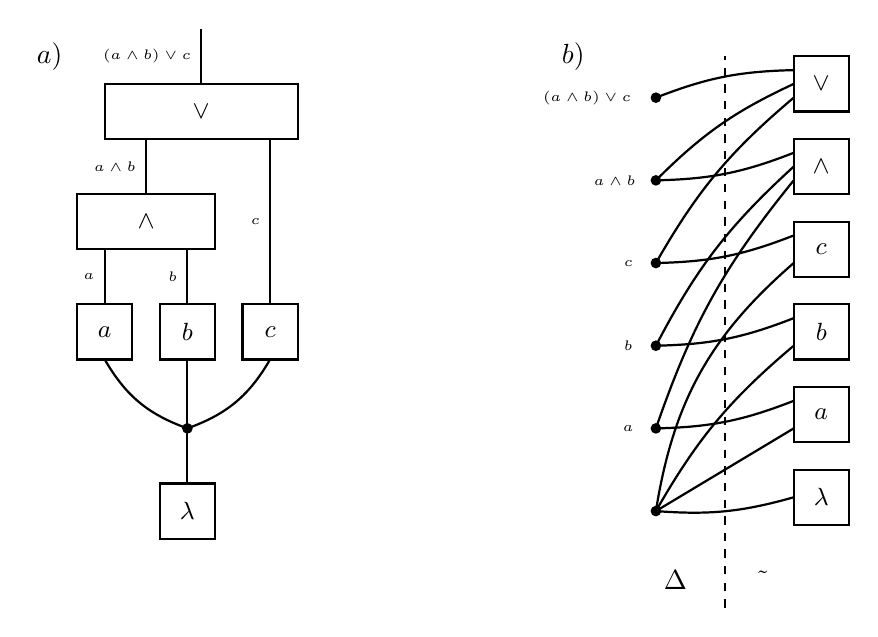
\begin{tikzpicture}[scale=0.35, thick] % , baseline = -3.5pt




\begin{scope}[shift={(23,0)}]

\node[anchor=center] (text) at (-6,8) {$b)$};

\draw (2,8) rectangle (4,6);
\node[anchor=center] (text) at (3,7) {\small $\bencodingof{\lor}$};

\draw (2,5) rectangle (4,3);
\node[anchor=center] (text) at (3,4) {\small $\bencodingof{\land}$};

\draw (2,2) rectangle (4,0);
\node[anchor=center] (text) at (3,1) {\small $\datacoreof{c}$};

\draw (2,-1) rectangle (4,-3);
\node[anchor=center] (text) at (3,-2) {\small $\datacoreof{b}$};

\draw (2,-4) rectangle (4,-6);
\node[anchor=center] (text) at (3,-5) {\small $\datacoreof{a}$};

\draw (2,-7) rectangle (4,-9);
\node[anchor=center] (text) at (3,-8) {\small $\lambda$};


\draw[fill] (-3,-8.5) circle (0.15cm);
\node[anchor=center] (text) at (-4,-8.5) {\tiny $\indexset$};

\draw[] (-3,-8.5) to[bend left=-10]  (2,-8);
\draw[] (-3,-8.5) to[bend left=0]  (2,-5.5);
\draw[] (-3,-8.5) to[bend left=10]  (2,-2.5);
\draw[] (-3,-8.5) to[bend left=20]  (2,0.5);


\draw[fill] (-3,-5.5) circle (0.15cm);
\node[anchor=center] (text) at (-4,-5.5) {\tiny $a$};

\draw[] (-3,-5.5) to[bend left=-10]  (2,-4.5);
\draw[] (-3,-5.5) to[bend left=10]  (2,3.5);

\draw[fill] (-3,-2.5) circle (0.15cm);
\node[anchor=center] (text) at (-4,-2.5) {\tiny $b$};

\draw[] (-3,-2.5) to[bend left=-10]  (2,-1.5);
\draw[] (-3,-2.5) to[bend left=10]  (2,4);

\draw[fill] (-3,0.5) circle (0.15cm);
\node[anchor=center] (text) at (-4,0.5) {\tiny $c$};

\draw[] (-3,0.5) to[bend left=-10]  (2,1.5);
\draw[] (-3,0.5) to[bend left=10]  (2,6.5);

\draw[fill] (-3,3.5) circle (0.15cm);
\node[anchor=center] (text) at (-4.5,3.5) {\tiny $a\land b$};

\draw[] (-3,3.5) to[bend left=-10]  (2,4.5);
\draw[] (-3,3.5) to[bend left=10]  (2,7);

\draw[fill] (-3,6.5) circle (0.15cm);
\node[anchor=center] (text) at (-5.5,6.5) {\tiny $(a\land b)\lor c$};

\draw[] (-3,6.5) to[bend left=10]  (2,7.5);


\draw[dashed] (-0.5,-12) -- (-0.5,8);

\node[right] (text) at (0.5,-11) {$\tilde{\edges}$};
\node[left] (text) at (-1.5,-11) {$\Delta$};

\end{scope}


\node[anchor=center] (text) at (-2,8) {$a)$};

\newcommand{\conposseldec}{3,-5.5}

\draw[fill] (\conposseldec) circle (0.15cm);
\draw (\conposseldec) -- (3,-7.5) node[midway, right] {\tiny ${\indexset}$}; % Unclear, whether this is the best notation!
\draw[] (2,-7.5) rectangle (4, -9.5);
\node[anchor=center] (text) at (3,-8.5) {\small $\lambda$};

\draw[] (0,1) -- (0,-1) node[midway,left] {\tiny $a$};
\draw (-1,-1) rectangle (1, -3);
\node[anchor=center] (text) at (0,-2) {\small $\datacoreof{a}$};
\draw[] (0,-3) to[bend right=20] (\conposseldec);


\draw[] (3,1) -- (3,-1) node[midway,left] {\tiny $b$};
\draw (2,-1) rectangle (4, -3);
\node[anchor=center] (text) at (3,-2) {\small $\datacoreof{b}$};
\draw[] (3,-3) to[bend right=0]  (\conposseldec);


\draw[] (6,5) -- (6,-1) node[midway,left] {\tiny $c$};
\draw (5,-1) rectangle (7, -3);
\node[anchor=center] (text) at (6,-2) {\small $\datacoreof{c}$};
\draw[] (6,-3) to[bend left=20]  (\conposseldec);


\draw[] (1.5,5) -- (1.5,3) node[midway,left] {\tiny $a \land b $};
\draw (-1,3) rectangle (4, 1);
\node[anchor=center] (text) at (1.5,2) {\small $\bencodingof{\land}$};


\draw[] (3.5,9) -- (3.5,7) node[midway,left] {\tiny $(a \land b) \lor c $};
\draw (0,7) rectangle (7, 5);
\node[anchor=center] (text) at (3.5,6) {\small $\bencodingof{\lor}$};

%\draw[] (6,1) to[bend left=20]  (\conposseldec);


		


\end{tikzpicture}
    \end{center}
    \caption{Example of a Bethe Cluster Graph.
    a) Example of a Tensor Network $\tnetof{\graph}$, which represents the by $\lambda$ averaged evaluation of the formula $(a\land b)\lor c$ on data $\datamap$.
    b) Corresponding Bethe Cluster Hypergraph, which dual is bipartite by the sets $\Delta$ and $\tilde{\edges}$.
    }
    \label{fig:betheDataExample}
\end{figure}





\subsection{Coarse graining}

\begin{definition}
    Let $\graph=(\nodes,\edges)$ and $\secgraph=(\node,\secedges)$ be two hypergraphs sharing their node set and $c: \edges \rightarrow \secedges$ a map.
    We say that $c$ is a coarse graining map and $\secgraph$, if for all $\edgein$
    \begin{align*}
        \edge \subset c(\edge) \, .
    \end{align*}
\end{definition}

In the literature such coarse graining procedures appear as Cluster Graphs.

\subsection{Variable Elimination}

Based on disjoint subsets of $\nodes$ we can construct a coarse graining procedure of a hypergraph:
Construct iteratively $\secedges$ by iterating through the node subsets and
\begin{itemize}
    \item Add those $\edge\in\edges$ which have not been assigned before and contain variables in the subset.
    \item Choose the new edge by the union of the old one with the assigned edges in $\edges$ and dropping those nodes, which are not appearing in the rest of $\edges$ any more.
    \item Return the intersection of the new edge with the rest of $\edges$ back to $\edges$.
\end{itemize}
By construction this gives a tree hypergraph.